% EPM-Bench --- ICLR 2027 submission draft
% NOTE: this file emulates the ICLR single-column format with standard
% packages so it compiles anywhere. For the real submission, drop in
% iclr2027_conference.sty and switch \documentclass line accordingly.
\documentclass[10pt]{article}
\usepackage[letterpaper,left=1.5in,right=1.5in,top=1in,bottom=1in]{geometry}
\usepackage{times}
\usepackage{graphicx}
\usepackage{booktabs}
\usepackage{amsmath,amssymb}
\usepackage{url}
\usepackage[small,compact]{titlesec}
\usepackage{caption}
\captionsetup{font=small,labelfont=bf}
\graphicspath{{results/}}
\setlength{\parskip}{2pt}

\newcommand{\todo}[1]{\textbf{\textcolor{red}{[TODO: #1]}}}
\usepackage{xcolor}

\title{\bf EPM-Bench: Benchmarking Prospective Memory\\
in Embodied Agents, Adjudicated from World State}
\author{Anonymous authors\\Paper under double-blind review}
\date{}

\begin{document}
\maketitle

\begin{abstract}
\noindent
Tell a household agent ``when you notice the kettle boiling, turn it off'' ---
then cancel the request. Will the agent still act? Agent memory research is
almost entirely \emph{retrospective}; no existing benchmark gives an embodied
agent a deferred instruction and adjudicates the full intention lifecycle
(acquisition, retention, execution, \emph{termination}) from world state, and
no prior work isolates the execution of cancelled intentions. We introduce
EPM-Bench, a dual-simulator benchmark (AI2-THOR kitchens, Habitat apartments)
of 7{,}564 frozen, procedurally generated episodes in which a seeded event
engine fires triggers outside the agent's field of view, every seed ships with
matched control / live / cancelled twins, and deterministic checkers grade
outcomes from simulator state alone --- no LLM judge anywhere. On the frozen
suite ($n{\ge}48$ per cell), commission errors are an \emph{architectural}
property of the memory pathway: a naively injected store executes 46--78\% of
cancelled intentions, while a typed store with mechanical revocation
bookkeeping eliminates violations at every window size, load, and simulator.
A window-bounded mock actor separates information starvation from attention
tax, establishing mechanical floors before any model is queried. A
grading-regime ablation over 1{,}440 cancelled intentions shows that
selection-style probes pass 52.9\% of agents that already violated in-world:
world-state adjudication is the only regime that grades the record rather
than the disposition. We release environments, the frozen suite, checkers,
validity probes, and traces.
\end{abstract}

\section{Introduction}

Embodied agents are beginning to hold obligations over time. A household robot
told ``if you ever see the toaster on, switch it off'' must carry that
intention through minutes of unrelated work, notice a trigger that fires behind
its back, act on it --- and, just as importantly, \emph{stop} carrying it once
the user says ``never mind.'' Human cognition treats this as a distinct memory
system: \emph{prospective memory} (PM), the memory for delayed intentions,
studied for three decades under monitoring cost, cue focality, intention load,
and \emph{commission errors} --- executing an intention after it has been
cancelled \citep{einstein1990, gollwitzer1999, virtualweek}.

Agent memory research has grown quickly, but in the \emph{retrospective}
direction: what did the agent see, where are objects, what happened yesterday
\citep{findingdory, memento, worldlines, robomemory, emem}. Text-side PM
benchmarks \citep{pmbench, triggerbench} grade deferred instructions by
question answering or menu selection rather than by what the agent does to the
world, and none places the trigger in an environment the agent must perceive.
Crucially, no prior work measures whether an agent executes an intention its
user has revoked.

This gap has a structural cause. QA-style and selection-style grading express
an agent's \emph{disposition} at probe time; a commission error lives in the
\emph{history} of the world. An agent that quietly turned off a cancelled
appliance ten steps ago will answer ``no, I should not act on it'' perfectly
well. We show this empirically in \S\ref{sec:grading}: a selection probe passes
52.9\% of agents that already violated.

We contribute:

\begin{enumerate}\itemsep2pt
\item \textbf{EPM-Bench}, the first execution-graded prospective-memory
benchmark in 3D worlds: deferred instructions injected mid-task, a seeded event
engine that changes the world out of view, per-step visibility instrumentation,
matched cancellation twins, and deterministic world-state checkers
(\S\ref{sec:bench}). The v0.1 suite is frozen: 7{,}564 episodes, 1{,}891 twin
groups, SHA-256 manifest, audited and bit-reproducible.
\item \textbf{EAC} (executed-after-cancellation) as a first-class metric,
calibrated by deaf-agent probes and common-sense controls
(\S\ref{sec:metrics}).
\item \textbf{Findings}: commission is manufactured or eliminated by the memory
pathway's bookkeeping, independent of model scale, intention load, and
simulator (\S\ref{sec:exp}); storing is easy, scheduling is the science.
\item \textbf{A mock-actor methodology} that separates information starvation
from attention tax, establishing mechanical floors before any token is spent
(\S\ref{sec:mech}).
\end{enumerate}

\section{Related Work}

\paragraph{Prospective memory for language agents.}
PM-Bench \citep{pmbench} adapts the Virtual Week paradigm to LLM agents over
simulated days; TriggerBench \citep{triggerbench} probes trigger--action
associations. Both grade text answers or option selection. Concurrent method
work introduces typed intention stores for small models
\citep{pis2026}, confirming that structured lifecycle logic helps --- but
evaluates on text benchmarks only and does not measure cancellation
compliance. Our benchmark supplies exactly the missing measurement.

\paragraph{Timing and proactivity.}
Gaia2 \citep{gaia2}, SentinelBench \citep{sentinel}, and SimuHome
\citep{simuhome} evaluate whether agents act at the right moment in simulated
schedules; they grade timeliness of live intentions, not the termination half
of the lifecycle.

\paragraph{Embodied memory.}
FindingDory \citep{findingdory}, MEMENTO \citep{memento}, and WorldLines
\citep{worldlines} benchmark retrospective memory in simulators; integrated
systems such as RoboMemory \citep{robomemory} and eMEM \citep{emem} ship
spatial, episodic, semantic, and temporal stores. Across 26 systems and
benchmarks we surveyed, no memory architecture contains a prospective store and
no benchmark contains a cancellation condition.

\paragraph{Termination neighbours.}
VIGIL \citep{vigil} isolates \emph{terminal commitment} --- whether an agent
correctly closes an episode --- decoupling world-state completion from reported
success. Chameleon \citep{chameleon} handles observation--action delay at the
control level for manipulation. Neither measures whether a revoked intention
stays dead.

\section{EPM-Bench}\label{sec:bench}

\subsection{Design principles}

\textbf{(P1) Full lifecycle in one episode.} Acquisition (a deferred
instruction arrives in the briefing alongside ongoing chores), retention
(interference from those chores), execution (the trigger fires out of view;
noticing must be earned), termination (matched cancelled variants;
exactly-once completion).

\textbf{(P2) World-state adjudication only.} Success and violation are computed
from simulator event logs by deterministic code. No LLM judge anywhere;
checkers ship with the benchmark.

\textbf{(P3) Memory isolated from common sense.} Every seed has a
no-instruction control twin. We report
$\mathrm{MEM} = \mathrm{EXEC}_{\text{live}} - \mathrm{EXEC}_{\text{control}}$.
This matters: a Haiku agent switches off a toaster it was never asked about in
30\% of control episodes.

\textbf{(P4) Noticing separated from acting.} Visibility is instrumented per
step (field of view, distance, occlusion), so failures are classified as
encoding / noticing / execution / termination.

\subsection{Environments}

\textbf{Kitchen tier (AI2-THOR).} Object-state triggers: a toaster, faucet, or
coffee machine is toggled on behind the agent's back by the event engine;
execution means the device is off in the final world state. Foreground chores
are pick-and-place errands. Ten kitchen scenes audited solvable (oracle 100\%).

\textbf{Apartment tier (habitat-sim).} Multi-room navigation; the trigger is a
marker that appears out of view; execution requires arriving \emph{and
declaring} (no accidental pass-by completions). Visibility is geometric: FOV
half-angle, distance, and a line-of-sight proxy. The marker carries no
common-sense meaning by design, which makes the control floor exactly zero and
isolates memory perfectly.

\subsection{Episodes and difficulty axes}

An episode is a tuple $\langle$scene, seed, chores, intentions, event schedule,
cancellation schedule, variant$\rangle$. Four matched variants per seed ---
\emph{control} (no intention briefed), \emph{live}, \emph{cancel-early}
(revocation before the event fires), \emph{cancel-late} (revocation after) ---
differ only in briefing and cancellation timing. Difficulty axes, all validated:
event delay (3--14 steps), intention load (1--3), cue focality (trigger on or
off the chore route), cancellation timing, scene scale (kitchen vs.\ apartment
vs.\ castle), and perception tier (privileged text vs.\ RGB).

\textbf{Frozen suite v0.1.} 6{,}000 THOR episodes (one dev kitchen, three
held-out kitchens) and 1{,}564 Habitat episodes (one dev apartment, one
held-out castle); 1{,}891 complete twin groups; SHA-256 manifest. Sampled
oracle audits pass on every scene; same-seed double runs produce bit-identical
event logs.

\subsection{Metrics and validity probes}\label{sec:metrics}

\textbf{EXEC}: fraction of live intentions executed exactly once.
\textbf{EAC} (headline): executed strictly after the revocation was delivered.
\textbf{MEM}: EXEC(live) $-$ EXEC(control).
\textbf{NOTICE}: first-visible-step vs.\ execution-step decomposition, giving
failure attribution shares (never-visible / visible-unnoticed /
noticed-unexecuted).
\textbf{COST}: steps, injected notes or tokens, foreground chores completed.

Three probes ship with the benchmark. A \emph{deaf} agent that cannot receive
cancellations calibrates EAC (its strict EAC equals its EXEC on early-cancel
arms: 47\% observed where honest agents score 0). \emph{Control twins} measure
the common-sense floor per scene and trigger. A \emph{determinism check}
verifies that same seed and policy produce identical event-log hashes.

\section{Experiments: mechanical layer}\label{sec:exp}

All cells in this section use $n{\ge}48$ episodes on the frozen suite.

\subsection{Reference agents reproduce human PM phenomena}

Scripted agents (oracle, negligent, opportunistic, periodic patroller,
adaptive patroller, deaf) mechanically reproduce the signatures of human
prospective memory. Monitoring has a foreground price and space sets the price:
periodic patrolling is strictly dominated by doing nothing extra in the
apartment tier. \emph{Where} to look beats \emph{how often}: coverage-greedy
vantage selection lifts execution from 70.8\% to 95.8\% at identical chore
cost. Incidental noticing decays with delay ($91.7 \to 25.0\%$ as the event
moves later) while disciplined monitoring degrades slowly. Intention load
degrades everything ($95.8 / 83.3 / 54.2\%$ for loads 1/2/3). Cue focality is
controllable: the same cue on vs.\ off the chore route yields 88.5\% vs.\ 40\%.
A one-line adaptive rule --- reset the monitoring clock on incidental sightings
--- collapses the entire fixed-frequency frontier to a single dominating point.

\subsection{The memory-policy triptych}

\begin{table}[t]
\centering\small
\caption{Frozen suite, THOR dev cell (delay 6, load 1, $n{=}50$ per arm).
EAC is reported separately for the early- and late-cancellation arms.
MEM is the memory contribution net of the control twin.}
\label{tab:headline}
\begin{tabular}{lccccc}
\toprule
Agent / memory policy & EXEC & CTRL & MEM & EAC (early) & EAC (late) \\
\midrule
Oracle (upper bound)        & 94.0 & --   & --   & 0.0  & 0.0 \\
Negligent (lower bound)     & 0.0  & --   & --   & 0.0  & 0.0 \\
Patroller ($k{=}6$)         & 94.0 & --   & --   & 0.0  & 0.0 \\
Adaptive patroller          & 94.0 & --   & --   & 0.0  & 0.0 \\
Deaf probe (validity)       & 94.0 & --   & --   & 47.0 & 0.0 \\
\midrule
No store                    & 0.0  & 0.0  & 0.0  & 0.0  & 0.0 \\
Naive always-injected store & 88.0 & 0.0  & 88.0 & 78.0 & 46.0 \\
Typed store + scheduler     & 58.0 & 0.0  & 58.0 & \bf 0.0 & \bf 0.0 \\
\bottomrule
\end{tabular}
\end{table}

A window-bounded rule actor --- it can act only on text inside its context
window --- makes the information boundary mechanical (Table~\ref{tab:headline},
Fig.~\ref{fig:triptych}). With no store, the briefing evicts and execution is
zero; window size acts as a dose ($0/0/29/63/67\%$ for $w{=}3\ldots48$). An
always-injected store pins the intention but lets the \emph{revocation} scroll
away: 88\% execution and 78\%/46\% executed-after-cancellation. A typed store
that strikes cancelled intentions from rotation and announces the strike once
achieves zero violations on both arms; its 30-point execution cost is the
resurfacing beat-gap (triggers sighted between scheduled reminders), the
mechanical face of the scheduling problem we pose in \S\ref{sec:mech}.

\begin{figure}[t]
\centering
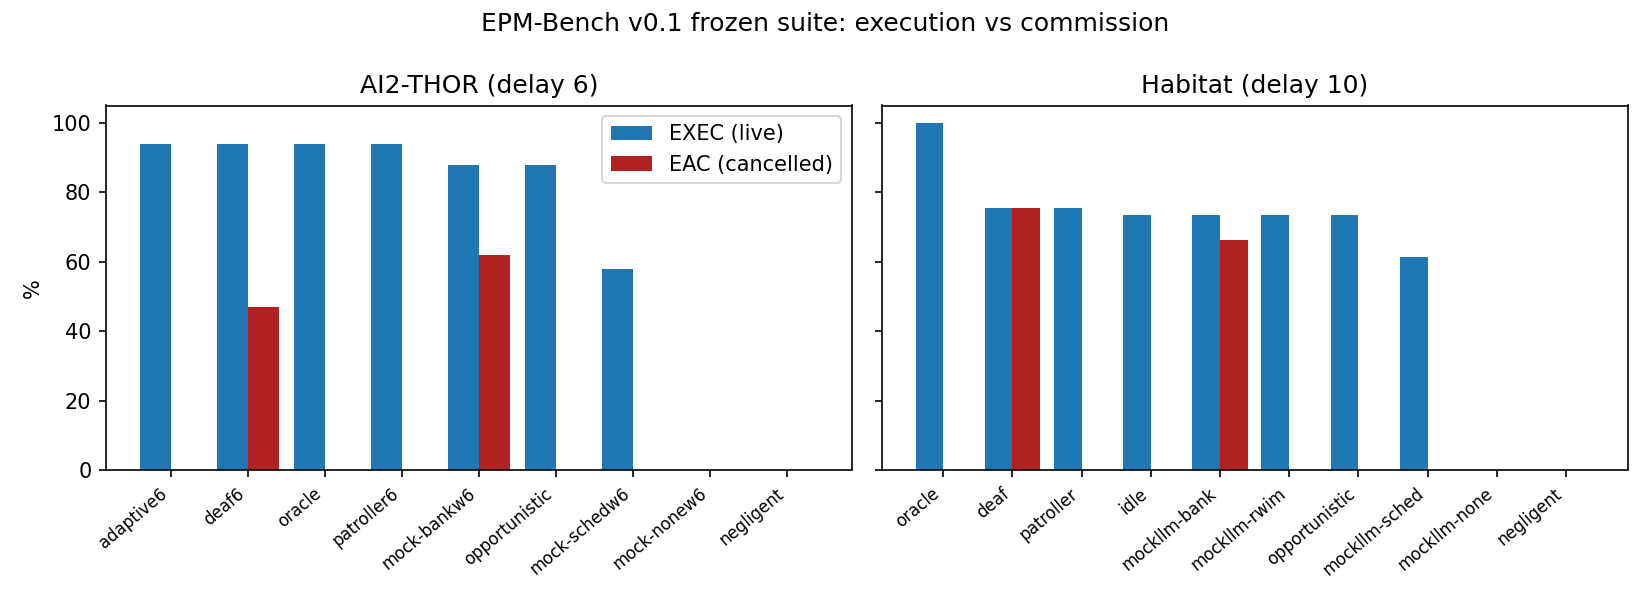
\includegraphics[width=.72\linewidth]{fig_suite_headline.png}
\caption{Headline cell of the frozen suite. Storing an intention is easy;
carrying its revocation is not.}
\label{fig:triptych}
\end{figure}

\subsection{Cancel-retention half-life, across engines}

The naive store's EAC falls monotonically with window size in both engines
(THOR: $71 \to 70 \to 61 \to 47 \to 18\%$ for $w{=}2,4,6,10,16$; Habitat:
$70 \to 68 \to 65 \to 64 \to 55\%$), while revocation-bookkeeping controls sit
at exactly 0\% at every window in both (Fig.~\ref{fig:window}). Commission is
window eviction plus schedule persistence --- reproducible without any model,
in any engine.

\begin{figure}[t]
\centering
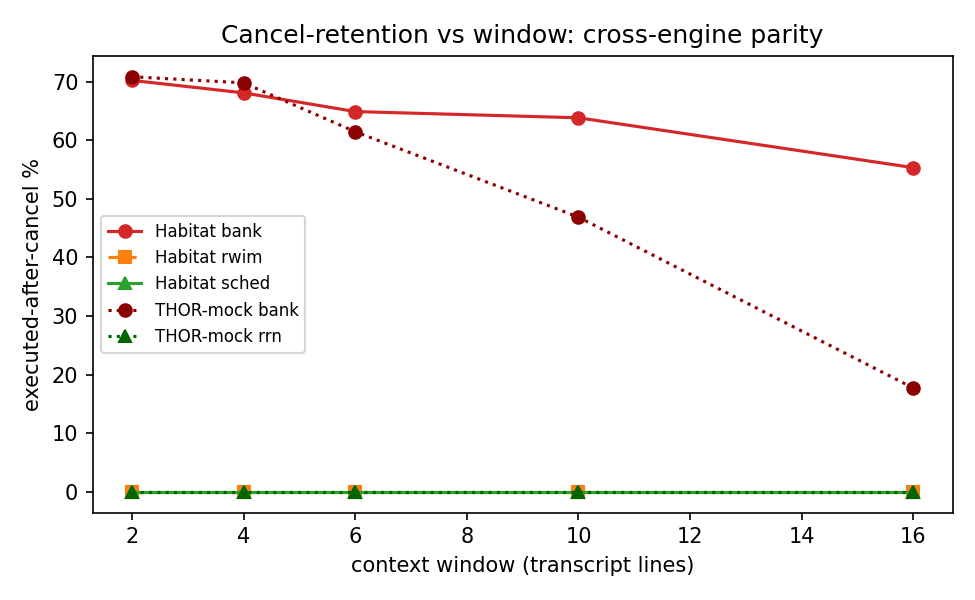
\includegraphics[width=.68\linewidth]{fig_window_parity.png}
\caption{Cancel-retention half-life. The naive store leaks less as the window
grows (the revocation survives longer); bookkeeping controls are pinned at zero
everywhere.}
\label{fig:window}
\end{figure}

\subsection{Generalization to held-out scenes}

On three held-out THOR kitchens the scripted ladder is unchanged (95.8\%), the
naive store drops to 68.1\% EXEC / 38.9\% EAC and the typed store to 48.6\% /
0.0\%: rankings invariant, absolutes scene-dependent. In the held-out Habitat
castle, patrolling collapses from 75.5\% to 29.2\% (the spatial-scale law)
while the oracle remains at 100\%, and the store ranking again holds
(45.8/41.7 vs.\ 25.0/0.0).

\section{Experiments: LLM tier}\label{sec:llm}

\emph{This section reports the August pilot ($n{=}8$--$20$ per arm, Claude
Haiku and Sonnet). The full grid ($n{\ge}50$, 2--3 model families, prompt
ablations, RGB at scale) is scripted and costed; results will replace these
numbers.} \todo{swap in solidification grid}

\textbf{Commission is real and architectural.} With a naive always-injected
store, Haiku executes cancelled intentions 70\% of the time in the kitchen and
60\% in the apartment. With a typed scheduled store, violations fall to the
common-sense floor (10\%) and to zero respectively, at one third of the token
cost.

\textbf{Scale does not buy prospective memory.} Sonnet's no-store execution
(37.5\%) exactly equals its no-intention control: its apparent memory is all
common sense. Commission softens but persists ($60 \to 37.5\%$), and the
ranking of memory policies is unchanged (Fig.~\ref{fig:scale}).

\textbf{Delegating the schedule to the model fails in structured ways.} A naive
LLM-coroutine memory manager emits 28--35 notes per 40 steps, all present-tense
chore micromanagement, never the deferred intention (10\% execution); a scoped
variant relabels chores as ``deferred intentions'' and leaves the real one
unguarded (30\%); actors also clock out with obligations open. Mechanical
resurfacing restores execution, but uniform resurfacing collapses under load
($90/30/20\%$ for loads 1/2/3) --- \emph{which} intention to resurface, and
when, is the open scheduling problem this benchmark poses cleanly.

\textbf{Perception costs points but preserves ranking.} Replacing privileged
text observations with raw RGB frames shifts every arm down by roughly 30
points while leaving the policy ordering intact.

\begin{figure}[t]
\centering
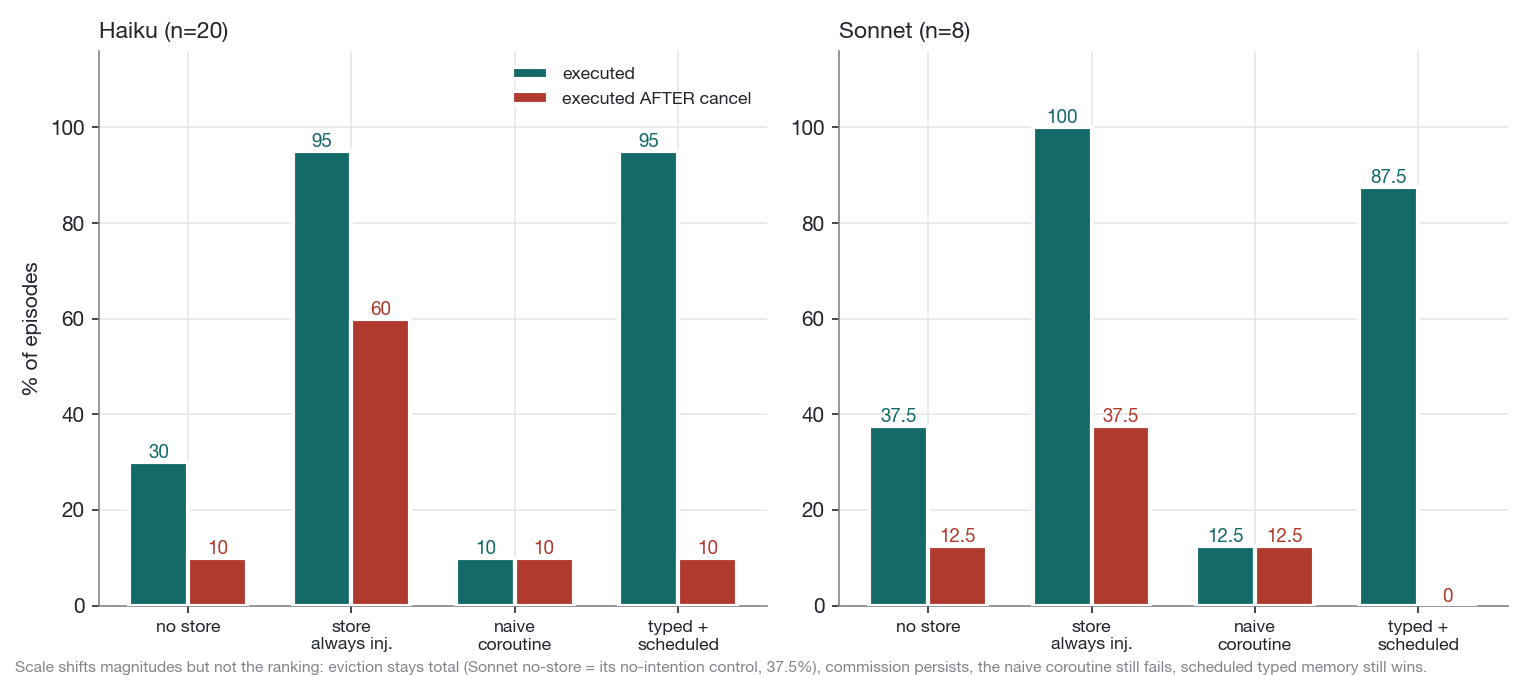
\includegraphics[width=.55\linewidth]{fig_model_scale.png}
\caption{Model scale does not change the memory-policy ranking (pilot).}
\label{fig:scale}
\end{figure}

\section{Mechanism: information floor versus attention tax}\label{sec:mech}

Because the mock actor has no attention limits, whatever it loses is
information starvation; whatever a real model loses beyond that is attention
tax. At load 3 the mechanical execution floor under full injection is 0.74 ---
every lost episode traces to a trigger that never entered the field of view on
the fixed chore route --- while the real Haiku scheduled agent sits at
0.20--0.30. The 40--50 point gap is an attention tax no injection schedule can
explain, and it motivates reporting EXEC conditioned on trigger visibility.

Two further mechanical facts constrain any future scheduler. First,
sight-triggered injection (inject a note only while its trigger is visible)
matches full injection's EXEC at every load for one fifth of the cost (22.8
vs.\ 120 notes per episode at load 3): mechanically it is the frontier. Yet
real models collapse on exactly this policy --- retrieval at cue onset arrives
too late without prior activation, the machine edition of the
implementation-intention effect \citep{gollwitzer1999}. Second, sparse
injection starves execution but also leaks fewer commissions than the naive
store (58\% vs.\ 75\% on the early arm): cost, execution, and compliance pull
in three directions \emph{before} any model enters the room.

\section{Grading-regime ablation}\label{sec:grading}

We grade the same 1{,}440 cancelled intentions (654 in-world violations) three
ways, giving each end-of-episode probe exactly the actor's information at the
final step. A selection-style probe (``would you act on this now?'') passes
\textbf{52.9\%} of violators: their disposition is clean by episode end, and the
violation lives in the history. A QA-style probe (``was this intention
cancelled?'') passes no violators but false-alarms on \textbf{63.4\%} of clean
episodes, because starved schedules leave nothing to recite even when no
violation occurred. World-state adjudication is the only regime that grades what
happened rather than what the agent would say (Fig.~\ref{fig:grading}). This is
the structural reason the termination half of the lifecycle has remained
unmeasured.

\begin{figure}[t]
\centering
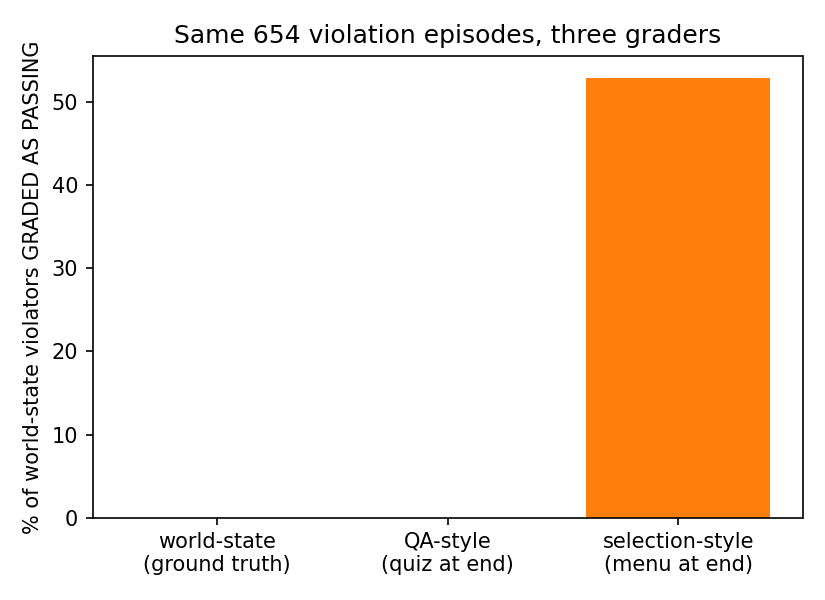
\includegraphics[width=.62\linewidth]{fig_grading_ablation.png}
\caption{Three graders, same episodes. Selection probes are blind to history;
QA probes false-alarm on clean episodes.}
\label{fig:grading}
\end{figure}

\section{Discussion}

An agent that executes revoked intentions is not merely forgetful; it is
disobedient in a way invisible to dialogue-level evaluation --- the interface
says ``okay'' while the world says otherwise. EAC gives this failure a number,
and the benchmark makes it cheap to measure. We view prospective memory as a
measurable, safety-relevant capability axis, and note that the same bookkeeping
that zeroes EAC also makes an agent's standing obligations inspectable by
humans, which is a prerequisite for oversight.

\section{Limitations}

LLM-tier numbers are pilot-scale pending the costed grid. Intentions are
single-user and explicit; inferred intentions are out of scope. Navigation is
teleport-based in the kitchen tier, and both tiers are simulators: our claims
live at the memory and decision layer, and sim-to-real transfer of low-level
control is not addressed. The late-cancel arm in the THOR tier coincides with
the fastest scripted response, which makes strict EAC definitionally zero for
step-8 responders on that one arm; v0.2 enforces a one-step gap. Finally, our
typed store is a reference implementation, not a proposed method: its 30-point
execution cost is a problem we pose rather than solve.

\section{Conclusion}

EPM-Bench turns ``remember to act --- and remember to stop'' into a measured,
reproducible quantity. Storing an intention is easy; scheduling it, and
scheduling its revocation, is the science. Commission errors are manufactured
or eliminated by the memory pathway's bookkeeping, independent of model scale
and simulator, and only world-state adjudication can see them. We release the
frozen suite, checkers, probes, and traces, and propose EAC as a standard
reporting axis for agent memory.

\subsubsection*{Reproducibility Statement}
The v0.1 suite is frozen and content-addressed: 7{,}564 episode specifications
are distributed as JSONL with a SHA-256 manifest, so that every reported cell
refers to identical episodes. Checkers are pure functions over simulator event
logs with unit tests on synthetic logs; no model is used for grading. A
determinism probe verifies bit-identical event logs across repeated runs of the
same seed and policy. Sampled oracle audits confirm every scene is solvable.
Environment wrappers, the episode generator, all reference agents, the analysis
scripts, and per-episode traces will be released.

\bibliographystyle{plainnat}
\begin{thebibliography}{20}\small
\bibitem[Einstein \& McDaniel(1990)]{einstein1990} G.~O. Einstein and M.~A.
McDaniel. Normal aging and prospective memory. \emph{JEP: LMC}, 1990.
\bibitem[Gollwitzer(1999)]{gollwitzer1999} P.~M. Gollwitzer. Implementation
intentions: strong effects of simple plans. \emph{American Psychologist}, 1999.
\bibitem[Rendell \& Craik(2000)]{virtualweek} P.~G. Rendell and F.~I.~M. Craik.
Virtual Week and actual week: age-related differences in prospective memory.
\emph{Applied Cognitive Psychology}, 2000.
\bibitem[PM-Bench(2026)]{pmbench} PM-Bench: evaluating prospective memory in
LLM agents. arXiv:2607.12385, 2026.
\bibitem[TriggerBench(2026)]{triggerbench} TriggerBench: investigating
prospective memory for large language models. arXiv:2606.23459, 2026.
\bibitem[Zhao \& Wu(2026)]{pis2026} J.~Zhao and C.~Wu. Making prospective
memory SLM-shaped: typed intention stores for small-model agents.
arXiv:2609.01272, 2026.
\bibitem[Gaia2(2025)]{gaia2} Gaia2: temporally grounded agent evaluation, 2025.
\bibitem[SentinelBench(2026)]{sentinel} SentinelBench: proactive monitoring
agents, 2026.
\bibitem[SimuHome(2026)]{simuhome} SimuHome: time-conditioned household agent
tasks, 2026.
\bibitem[FindingDory(2026)]{findingdory} FindingDory: benchmarking embodied
agent memory. ECCV, 2026.
\bibitem[MEMENTO(2026)]{memento} Embodied agents meet personalization:
investigating challenges through the lens of memory utilization. ICLR, 2026.
\bibitem[WorldLines(2026)]{worldlines} WorldLines: benchmarking and modeling
long-horizon stateful embodied agents. arXiv:2606.18847, 2026.
\bibitem[RoboMemory(2025)]{robomemory} RoboMemory: a brain-inspired multi-memory
framework for embodied agents. arXiv:2508.01415, 2025.
\bibitem[eMEM(2026)]{emem} eMEM: hippocampus-inspired spatio-temporal memory
for embodied agents. arXiv:2606.03374, 2026.
\bibitem[VIGIL(2026)]{vigil} Done, but not sure: disentangling world completion
from self-termination in embodied agents. arXiv:2605.08747, 2026.
\bibitem[Chameleon(2026)]{chameleon} Chameleon: control-indexed prospective
memory for visuomotor manipulation. arXiv:2603.24576, 2026.
\bibitem[AI2-THOR(2017)]{thor} AI2-THOR: an interactive 3D environment for
visual AI. arXiv:1712.05474, 2017.
\bibitem[Habitat(2019)]{habitat} Habitat: a platform for embodied AI research.
ICCV, 2019.
\end{thebibliography}

\end{document}
